% GNUPLOT: LaTeX picture with Postscript
\begingroup
  \makeatletter
  \providecommand\color[2][]{%
    \GenericError{(gnuplot) \space\space\space\@spaces}{%
      Package color not loaded in conjunction with
      terminal option `colourtext'%
    }{See the gnuplot documentation for explanation.%
    }{Either use 'blacktext' in gnuplot or load the package
      color.sty in LaTeX.}%
    \renewcommand\color[2][]{}%
  }%
  \providecommand\includegraphics[2][]{%
    \GenericError{(gnuplot) \space\space\space\@spaces}{%
      Package graphicx or graphics not loaded%
    }{See the gnuplot documentation for explanation.%
    }{The gnuplot epslatex terminal needs graphicx.sty or graphics.sty.}%
    \renewcommand\includegraphics[2][]{}%
  }%
  \providecommand\rotatebox[2]{#2}%
  \@ifundefined{ifGPcolor}{%
    \newif\ifGPcolor
    \GPcolortrue
  }{}%
  \@ifundefined{ifGPblacktext}{%
    \newif\ifGPblacktext
    \GPblacktextfalse
  }{}%
  % define a \g@addto@macro without @ in the name:
  \let\gplgaddtomacro\g@addto@macro
  % define empty templates for all commands taking text:
  \gdef\gplbacktext{}%
  \gdef\gplfronttext{}%
  \makeatother
  \ifGPblacktext
    % no textcolor at all
    \def\colorrgb#1{}%
    \def\colorgray#1{}%
  \else
    % gray or color?
    \ifGPcolor
      \def\colorrgb#1{\color[rgb]{#1}}%
      \def\colorgray#1{\color[gray]{#1}}%
      \expandafter\def\csname LTw\endcsname{\color{white}}%
      \expandafter\def\csname LTb\endcsname{\color{black}}%
      \expandafter\def\csname LTa\endcsname{\color{black}}%
      \expandafter\def\csname LT0\endcsname{\color[rgb]{1,0,0}}%
      \expandafter\def\csname LT1\endcsname{\color[rgb]{0,1,0}}%
      \expandafter\def\csname LT2\endcsname{\color[rgb]{0,0,1}}%
      \expandafter\def\csname LT3\endcsname{\color[rgb]{1,0,1}}%
      \expandafter\def\csname LT4\endcsname{\color[rgb]{0,1,1}}%
      \expandafter\def\csname LT5\endcsname{\color[rgb]{1,1,0}}%
      \expandafter\def\csname LT6\endcsname{\color[rgb]{0,0,0}}%
      \expandafter\def\csname LT7\endcsname{\color[rgb]{1,0.3,0}}%
      \expandafter\def\csname LT8\endcsname{\color[rgb]{0.5,0.5,0.5}}%
    \else
      % gray
      \def\colorrgb#1{\color{black}}%
      \def\colorgray#1{\color[gray]{#1}}%
      \expandafter\def\csname LTw\endcsname{\color{white}}%
      \expandafter\def\csname LTb\endcsname{\color{black}}%
      \expandafter\def\csname LTa\endcsname{\color{black}}%
      \expandafter\def\csname LT0\endcsname{\color{black}}%
      \expandafter\def\csname LT1\endcsname{\color{black}}%
      \expandafter\def\csname LT2\endcsname{\color{black}}%
      \expandafter\def\csname LT3\endcsname{\color{black}}%
      \expandafter\def\csname LT4\endcsname{\color{black}}%
      \expandafter\def\csname LT5\endcsname{\color{black}}%
      \expandafter\def\csname LT6\endcsname{\color{black}}%
      \expandafter\def\csname LT7\endcsname{\color{black}}%
      \expandafter\def\csname LT8\endcsname{\color{black}}%
    \fi
  \fi
  \setlength{\unitlength}{0.0500bp}%
  \begin{picture}(11338.00,5102.00)%
      \csname LTb\endcsname%
      \put(5669,4882){\makebox(0,0){\strut{}Doppelpendel}}%
    \gplgaddtomacro\gplbacktext{%
      \csname LTb\endcsname%
      \put(946,890){\makebox(0,0)[r]{\strut{}-2}}%
      \put(946,1414){\makebox(0,0)[r]{\strut{}-1.5}}%
      \put(946,1938){\makebox(0,0)[r]{\strut{}-1}}%
      \put(946,2463){\makebox(0,0)[r]{\strut{}-0.5}}%
      \put(946,2987){\makebox(0,0)[r]{\strut{} 0}}%
      \put(946,3511){\makebox(0,0)[r]{\strut{} 0.5}}%
      \put(946,4035){\makebox(0,0)[r]{\strut{} 1}}%
      \put(1078,670){\makebox(0,0){\strut{}-2}}%
      \put(1602,670){\makebox(0,0){\strut{}-1.5}}%
      \put(2127,670){\makebox(0,0){\strut{}-1}}%
      \put(2651,670){\makebox(0,0){\strut{}-0.5}}%
      \put(3175,670){\makebox(0,0){\strut{} 0}}%
      \put(3699,670){\makebox(0,0){\strut{} 0.5}}%
      \put(4224,670){\makebox(0,0){\strut{} 1}}%
      \put(4748,670){\makebox(0,0){\strut{} 1.5}}%
      \put(5272,670){\makebox(0,0){\strut{} 2}}%
      \put(176,2462){\rotatebox{-270}{\makebox(0,0){\strut{}Position $y$ [m]}}}%
      \put(3175,340){\makebox(0,0){\strut{}Position $x$ [m]}}%
      \put(3175,4365){\makebox(0,0){\strut{}Trajektorie}}%
    }%
    \gplgaddtomacro\gplfronttext{%
    }%
    \gplgaddtomacro\gplbacktext{%
      \csname LTb\endcsname%
      \put(6351,791){\makebox(0,0)[r]{\strut{}-8}}%
      \put(6351,1209){\makebox(0,0)[r]{\strut{}-6}}%
      \put(6351,1627){\makebox(0,0)[r]{\strut{}-4}}%
      \put(6351,2045){\makebox(0,0)[r]{\strut{}-2}}%
      \put(6351,2463){\makebox(0,0)[r]{\strut{} 0}}%
      \put(6351,2880){\makebox(0,0)[r]{\strut{} 2}}%
      \put(6351,3298){\makebox(0,0)[r]{\strut{} 4}}%
      \put(6351,3716){\makebox(0,0)[r]{\strut{} 6}}%
      \put(6351,4134){\makebox(0,0)[r]{\strut{} 8}}%
      \put(6483,571){\makebox(0,0){\strut{}-2.5}}%
      \put(6888,571){\makebox(0,0){\strut{}-2}}%
      \put(7294,571){\makebox(0,0){\strut{}-1.5}}%
      \put(7699,571){\makebox(0,0){\strut{}-1}}%
      \put(8104,571){\makebox(0,0){\strut{}-0.5}}%
      \put(8509,571){\makebox(0,0){\strut{} 0}}%
      \put(8915,571){\makebox(0,0){\strut{} 0.5}}%
      \put(9320,571){\makebox(0,0){\strut{} 1}}%
      \put(9725,571){\makebox(0,0){\strut{} 1.5}}%
      \put(10130,571){\makebox(0,0){\strut{} 2}}%
      \put(10536,571){\makebox(0,0){\strut{} 2.5}}%
      \put(10941,571){\makebox(0,0){\strut{} 3}}%
      \put(5845,2462){\rotatebox{-270}{\makebox(0,0){\strut{}kanonisch konjugierter Impuls $p_{\theta}$}}}%
      \put(8712,241){\makebox(0,0){\strut{}Auslenkung $\theta$}}%
      \put(8712,4464){\makebox(0,0){\strut{}Phasenraum}}%
    }%
    \gplgaddtomacro\gplfronttext{%
    }%
    \gplbacktext
    \put(0,0){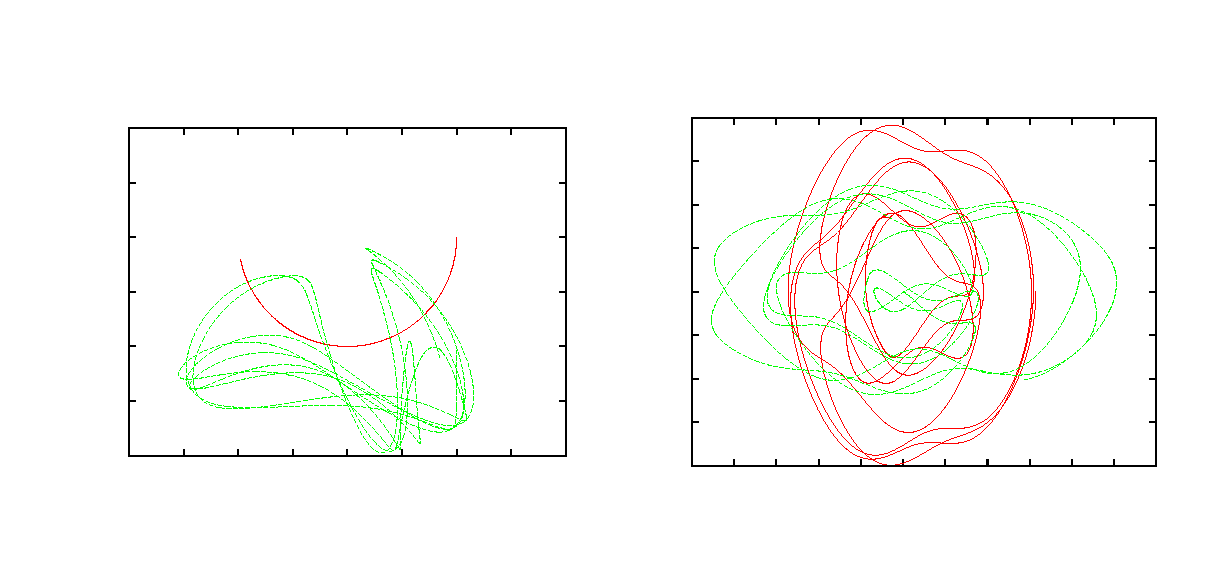
\includegraphics{./figures/trajektorie}}%
    \gplfronttext
  \end{picture}%
\endgroup
